\chapter{Návrh a architektura aplikace}

\section{Serverová část}

Rozdělení do projektů:

TODO: u každé dopodrobna rozepsat co obsahuje, k čemu slouží + ukázky kódu

\subsection{Data}

Tento projekt se stará primárně o komunikaci s databází, pro tento účel jsme použili ORM framework Entity Framework Core. 

Ve složce Models jsou třídy reprezentující databázové entity. Každá z entit pak v databázi představuje jednu tabulku. V aplikaci jsme použili tyto entity:

\begin{table}[ht]
	\centering
	\begin{tabular}{| l | p{9cm} |}
		\hline
		Název entity & reprezentuje \\
		\hline \hline
		Course & kurz \\ \hline
		CourseFile & nějaký soubor sdílený v kurzu \\ \hline
		CourseMember & členství uživatele v daném kurzu. 
		K této entitě se pak vážou všechny známky a odeslané testy. \\ \hline
		CourseTest & test v kurzu \\ \hline
		ForumPost & příspěvek ve fóru k danému kurzu \\ \hline
		Grade & známku kterou student obdržel (kromě známek z testů) \\ \hline
		Person & uživatele aplikace \\ \hline
		TestQuestion & 1 otázku v testu \\ \hline
		TestSubmission & test s odpověďmi odeslaný uživatelem \\ \hline
		TestSubmissionAnswer & odpověď k dané otázce v testu \\
		\hline
	\end{tabular}
\end{table}

\newpage

\begin{figure}
	\centering
	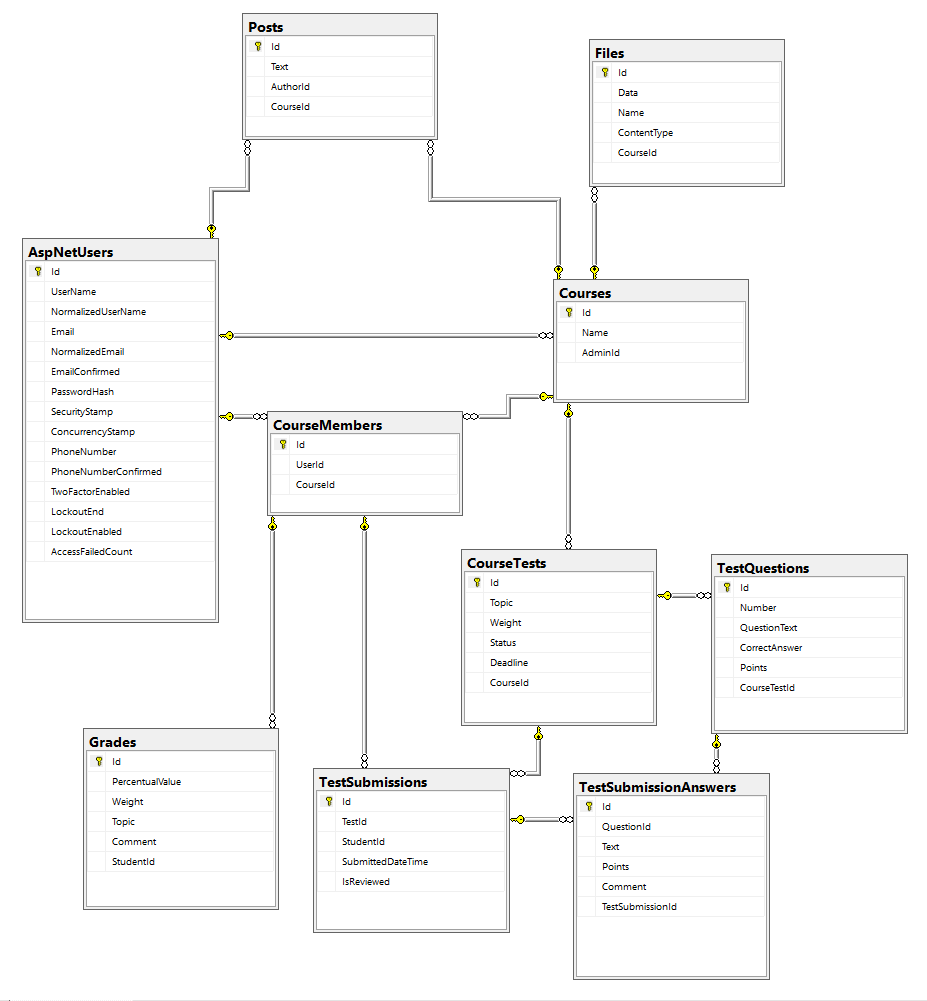
\includegraphics[width=\textwidth]{db_model.PNG}
	\caption{Databázový model aplikace}
\end{figure}

\newpage

např. kód třídy Course vypadá takto:

\begin{lstlisting}
public class Course : IGuidIdObject
{
	public Course()
	{
		Members = new List<CourseMember>();
		Files = new List<CourseFile>();
		Tests = new List<CourseTest>();
		ForumPosts = new List<ForumPost>();
	}
	
	public Course(string name, Person admin) : this()
	{
		Name = name;
		Admin = admin;
	}
	
	/// <summary>
	/// identifier of the couse
	/// </summary>
	[DatabaseGenerated(DatabaseGeneratedOption.Identity)]
	[Key]
	public Guid Id { get; set; }
	
	/// <summary>
	/// name of the course
	/// </summary>
	[Required]
	public string Name { get; set; }
	
	...
\end{lstlisting}

Vidíme, že každá entita obsahuje veřejné vlastnosti (public properties) s gettery a settery. Tyto vlastnosti budou v databázové tabulce reprezentovány jako sloupce. Některé z nich (jako např. Id) obsahují ještě doplňující atributy, ty slouží k upřesnění informací o dané vlastnosti. Například atribut [Key] určuje, že tato vlastnost bude v databázi primární klíč, atribut [Required] určuje, že daný sloupec bude v tabulce u všech záznamů povinný (tedy hodnoty budou NOT NULL).
Dále musí každá entita obsahovat konstruktor bez parametrů.

Vazby mezi entitami jsou reprezentované pomocí tzv. navigačních vlastností. V případě, že chceme vytvořit vazbu typu one-to-many mezi entitami A a B, stačí do vlastností třídy A přidat kolekci objektů typu B, a naopak do třídy B vlastnost typu A. Framework pak při provádění migrace vytvoří v databázové tabulce entity B vytvoří sloupec s cizím klíčem, který bude obsahovat identifikátor entity A, ke které patří.

V aplikaci je vazba one-to-many použita mimo jiné mezi entitami Course a CourseTest, a to tak, že každý test je obsažen v právě jednom kurzu, a v daném kurzu může být N testů.
Kód pak tedy vypadá takto: ve třídě Course je kolekce objektů typu CourseTest

\begin{lstlisting}
/// <summary>
/// tests in this course
/// </summary>
public ICollection<CourseTest> Tests { get; set; }
\end{lstlisting}

a ve třídě CourseTest je pak vlastnost typu Course

\begin{lstlisting}
/// <summary>
/// course that contains this test
/// </summary>
[Required]
public Course Course { get; set; }
\end{lstlisting}

Po provedení databázové migrace (viz. dále) se v tabulce CourseTest vytvoří sloupec CourseId s cizím klíčem, který odkazuje na identifikátor kurzu (tzn. vlastnost Course.Id).

Také si můžeme všimnout, že všechny entity (kromě entity Person) implementují rozhraní IGuidObject. To je jednoduché rozhraní, které obsahuje pouze jednu vlastnost - Id typu Guid. Tímto máme zajištěnou jednotu identifikátorů, tedy že všechny entity, které toto rozhraní implementují, budou mít identifikátor typu Guid.

\begin{lstlisting}
/// <summary>
/// interface for object with <see cref="Guid"/> identifier
/// </summary>
public interface IGuidIdObject
{
	/// <summary>
	/// identifier of the object
	/// </summary>
	Guid Id { get; set; }
}
\end{lstlisting}


Typ Guid jsme zvolili hlavně z toho důvodu, že vestavěné tabulky frameworku (např. Identity) mají také řetězcové identifikátory. Navíc se pak zjednoduší práce ve frontend části (není potřeba parsovat string na int např. v klientské části při práci s URL). Tyto identifikátory generuje databáze, takže je zajištěno, že jsou unikátní.
Další možnost by byla použít jako identifikátor číslo (např. typ int), ale vzhledem k výše uvedeným argumentům je typ Guid v tomto případě lepší možnost.

Dále se v projektu nachází také rozhraní ICourseReferenceObject a ICourseMemberReferenceObject, které slouží k tomu, abychom mohli dále v aplikaci jednotně pracovat s objekty, které mají referenci na entitu Course, resp. CourseMember. Tyto rozhraní implementují pouze nějaké entity.

V programu je dále třída CMSDbContext, která reprezentuje databázový kontext této aplikace. Každý objekt typu DbSet pak představuje jednu databázovou tabulku. Ve třídě je CMSDbContext tedy kolekce typu DbSet pro každou z entit.

\begin{lstlisting}
public DbSet<Grade> Grades { get; set; }

public DbSet<Course> Courses { get; set; }

...
\end{lstlisting}

Jediná výjimka je entita Person, která dědí ze třídy IdentityUser, a jejíž DbSet je nakonfigurovaný ve frameworku. 

V programu pak dále používáme ke komunikaci s databází pouze třídu CMSDbContext a objekty typu DbSet. Třida DbSet<TEntity> implementuje rozhraní IQueryable<TEntity>, takže na ní lze použít LINQ. Takže pokud bych chtěl například vybrat všechny kurzy, jejiž jméno začíná na písmeno C, pak stačí použít následující LINQ dotaz
\begin{lstlisting}
dbContext.Courses.Where(course => course.Name.StartsWith("C"))
\end{lstlisting}
kde proměnná dbContext je instance třídy CMSDbContext.

Ve třídě CMSDbContext je také metoda ConfigureForeignKeys, která provede konfiguraci cizích klíčů v aplikaci. Všechny políčka s cizími klíči jsou v databázi povinné (tzn. NOT NULL), to je zajištěno pomocí atributu [Required] daných vlastností. Nastavením DeleteBehavior.Restrict u cizích klíčů zajistíme, že databáze zůstane v konzistentním stavu. Pokud bychom tedy chtěli smazat entitu, pak na ní nesmí pomocí cizích klíčů odkazovat jiné entity. V opačném případě program při zavolání metody SaveChanges() na databázovém kontextu vyhodí výjimku.

V programu je dále složka Migrations. Při vývoji byl použit princip Code first, tedy že v kódu specifikujeme entity pomocí klasických tříd. Framework se pak postará o vytvoření databázových tabulek z tohoto kódu.

Pokud jsem tedy nějak změníme některou z entit (to může být např. přidání vlastnosti, změna jména vlastnosti, apod.), pak pomocí ORM můžeme vygenerovat soubor popisující tzv. databázovou migraci, která slouží k aplikaci změn z kódu do databáze. Ke každé migraci se vygeneruje jeden soubor, který obsahuje popis změn, které se později provedou v databázi.

K vytváření migrací jsem použijeme nástroj CLI tools for Entity Framework Core. https://docs.microsoft.com/cs-cz/ef/core/cli/dotnet. Pro vygenerování migrace ze změn v kódu použijeme příkaz:

TO-Do: přesunout přesný příkaz jinam

\begin{lstlisting}
dotnet ef migrations add {migration_name} 
--project CourseManagementSystem.Data 
--startup-project CourseManagementSystem.API
\end{lstlisting}

Tímto se vytvoří soubor popisující změny v migraci, ale databáze zatím zůstala beze změny. Tento soubor obsahuje třídu, jenž dědí ze třídy Migration a obsahuje metody Up a Down. V metodě Up je popis změn, které se provedou při aplikaci této migrace, naopak v metodě Down je popis změn, které se provedou v případě odstranění migrace.

Jako příklad si můžeme představit migraci, která obsahuje přidání vlastnosti ScoreWeight k entitě CourseTest (tato vlastnost popisuje váhu testu).
Vygenerovaný kód migrace vypadá takto:

\begin{lstlisting}
public partial class TestWeight_added : Migration
{
	protected override void Up(MigrationBuilder migrationBuilder)
	{
		migrationBuilder.AddColumn<int>(
		name: "ScoreWeight",
		table: "CourseTests",
		nullable: false,
		defaultValue: 0);
	}
	
	protected override void Down(MigrationBuilder migrationBuilder)
	{
		migrationBuilder.DropColumn(
		name: "ScoreWeight",
		table: "CourseTests");
	}
}
\end{lstlisting}

TO-DO: přesunout syntaxi příkaz jinam

Pro promítnutí změn do databáze následně použijeme příkaz:

\begin{lstlisting}
dotnet ef database update 
--project CourseManagementSystem.Data 
--startup-project CourseManagementSystem.API
\end{lstlisting}

Tímto tedy dojde k změnám v databázi (v našem příkladu se vytvoří sloupec ScoreWeight v tabulce CourseTests).

V obou příkazech je potřeba specifikovat cílový a startup projekt. Cílový projekt je ten, který obsahuje databázový kontext a entity naší aplikace (v tomto případě projekt Data). Naopak startup projekt je projekt, který je spouštěný frameworkem, což je potřeba pro získání konfiguračních informací o projektu, jako je například connection string do naší databáze.

\newpage

\subsection{Services}
V tomto projektu se nachází pomocné služby pro komunikaci s databází. 

Jako základ pro všechny služby slouží abstraktní třída DbService, která obsahuje referenci na databázový kontext aplikace a jedinou metodu CommitChanges(). Ta slouží k uložení změn provedených v databázovém kontextu do databáze. 

To je potřeba, protože k uložení změn do databáze dojde až tehdy, když na databázovém kontextu zavoláme metodu SaveChanges(). Pokud bychom tedy například do databázového kontextu něco uložili (např. takto: 
\begin{lstlisting}
dbContext.Grades.Add(new Grade())
\end{lstlisting}
a nezavolali metodu dbContext.SaveChanges(), data by se neuložila.

\begin{lstlisting}
/// <summary>
/// class representing base database service
/// </summary>
public abstract class DbService : IDbService
{
	/// <summary>
	/// context of the CMS database
	/// </summary>
	protected readonly CMSDbContext dbContext;
	
	/// <summary>
	/// construct a new database service
	/// </summary>
	/// <param name="dbContext">CMS database context</param>
	protected DbService(CMSDbContext dbContext)
	{
		this.dbContext = dbContext;
	}
	
	/// <inheritdoc/>
	public void CommitChanges()
	{
		dbContext.SaveChanges();
	}
}
\end{lstlisting}

Tato třída implementuje rozhraní IDbService, které obsahuje pouze metodu CommitChanges().

Dále jsou ve složce Interfaces rozhraní pro další služby, ty jsou rozdělené podle entit (typicky máme pro jednu entitu jednu službu). Všechny tyto rozhraní také implementují rozhraní IDbService. 

Například rozhraní ICourseService (slouží pro práci s kurzy) vypadá takto:
\begin{lstlisting}
public interface ICourseService : IDbService
{
	/// <summary>
	/// get course by its id
	/// </summary>
	/// <param name="courseId">identifier of the course</param>
	/// <returns></returns>
	Course GetById(string courseId);
	
	/// <summary>
	/// archive course by its id
	/// </summary>
	/// <param name="courseId">id of the course to delete</param>
	void ArchiveById(string courseId);
	
	/// <summary>
	/// add the course into the database
	/// </summary>
	/// <param name="course">course to add</param>
	void AddCourse(Course course);
	...
\end{lstlisting}

Ve složce Implementations jsou potom implementace těchto rozhraní. Můžeme vidět, že všechny implementace dědí ze třídy DbService, a zároveň také tranzitivně implementují IDbService.

Například třída CourseService, která implementuje rozhraní ICourseService vypadá takto:

\begin{lstlisting}
public class CourseService : DbService, ICourseService
{
	public CourseService(CMSDbContext dbContext) : base(dbContext)
	{ }
	
	/// <inheritdoc/>
	public void ArchiveById(string courseId)
	{
		Course c = GetById(courseId);
		c.IsArchived = true;
	}
	
	/// <inheritdoc/>
	public Course GetById(string courseId)
	{
		return dbContext.Courses.FindById(courseId);
	}
	
	/// <inheritdoc/>
	public void AddCourse(Course course)
	{
		dbContext.Courses.Add(course);
	}
	...
\end{lstlisting}

Vidíme, že služby typicky pracují s databázovým kontextem, a s daty (vyhledávání, mazání, apod.).
Dále si můžeme všimnout, že v žádné metodě se neukládájí změny do databáze (tzn. volání metody CommitChanges()). To je z toho důvodu, že ve vyšších vrstvách aplikace (např. API) v jedné metodě často voláme několik služeb, příp. několik metod z jedné služby. 
Pokud bychom v metodách služeb přímo ukládali změny do databáze (metoda CommitChanges()), pak bychom se mohli lehce dostat to nekonzistentního stavu. To například tak, že při volání několika služeb v rámci jedné metody by 
mohla některá ze služeb vyhodit výjimku, nicméně všechny služby zavolané předtím by už data uložily.

Takže je na zodpovědnosti volajícího provést uložení změn do databáze, tedy zavolat metodu CommitChanges(), což je typicky poslední příkaz v dané metodě.
Tím jsme tedy zajistili konzistenci dat - buď se do databáze uloží všechny změny provedené v databázovém kontextu, nebo žádné.

Dále si můžeme všimnout, že ve službách pracujeme s identifikátory typu string, ale v databázi používáme typ Guid. To je z toho důvodu, že ve vyšších vrstvách aplikace se pohodlněji pracuje se stringy (např. často dostáváme ID jako URL parametr). Převod mezi typy string a Guid pak řešíme ve službách.

Ve složce Extensions jsou pak pomocné extension metody pro práci s některými třídami.

Ve třídě DbSetExtensions se nachází extension metody pro třídu DbSet<T>. Vybereme si například metodu GetCourseIdOf, ta slouží k získání ID kurzu, ke kterému daný objekt, jenž má referenci na entitu Course, patří.
\begin{lstlisting}
/// <summary>
/// get id of <see cref="Data.Models.Course"/> that the object belongs to
/// </summary>
/// <typeparam name="T">type of items</typeparam>
/// <param name="dbSet">database set</param>
/// <param name="objectId">identifier of the object we look for in <paramref name="dbSet"/></param>
/// <returns></returns>
public static string GetCourseIdOf<T>(this DbSet<T> dbSet, string objectId) where T : class, ICourseReferenceObject, IGuidIdObject
{
	return dbSet.Include(item => item.Course)
		.Single(item => item.Id.ToString() == objectId)
		.Course.Id.ToString();
}
\end{lstlisting}

Vidíme, že toto je jeden z příkladů použití rozhraní ICourseReferenceObject, které se nachází v projektu Data.

V projektu též máme rozhraní ICourseReferenceService, to implementují všechny služby, jejichž entity logicky patří k nějakému kurzu. Rozhraní obsahuje jedinou metodu GetCourseIdOf(string objectId), která získá ID kurzu, ke kterému daná entita patří. V implementaci této metodu pak typicky používáme extension metodu GetCourseIdOf pro třídu DbSet<T>. Například ve třídě CourseTestService vypadá implementace takto:

\begin{lstlisting}
public string GetCourseIdOf(string objectId)
{
	return dbContext.CourseTests.GetCourseIdOf(objectId);
}
\end{lstlisting}

Podobně je v projektu i rozhraní ICourseMemberReferenceService, které používají služby, jejichž entity mají referenci na třídu CourseMember.

Použitím služeb jsme odstranili duplikátní kód (např. hledání kurzu podle ID se používá na několika místech ve vyšších vrstvách), a extrahovali některé složitější dotazy do samostatných metod. To je výhodné hlavně z toho důvodu, že je pak můžeme nezávisle otestovat. Další výhoda je, že vyšší vrstvy jsou odstíněny od použití ORM (a databázového kontextu), pouze volají tyto služby.

Dále si můžeme všimnout, že ve službách používáme při komunikaci s databázovým kontextem tzv. Eager loading (pomocí metod Include()). To znamená, že data databázových entit které daná entita referencuje, se při výchozím chování nenačtou (pokud nepoužijeme metodu Include), tzn. budou mít hodnotu NULL.

Například pro získání testu s otázkami můžeme použít tento příkaz:
\begin{lstlisting}
dbContext.CourseTests
	.Include(test => test.Questions)
\end{lstlisting}
Pokud bych volání metody Include() vynechal, tak by se data otázek nenačetla.

\newpage

\subsection{API}
V tomto projektu se nachází API, které slouží pro komunikaci klientské části se serverovou.

\subsubsection*{Controllers}
Controllery slouží primárně ke zpracování HTTP požadavků. Vidíme, že Controller je klasická C\# třída, jenž dědí ze třídy ControllerBase. Ve většině případů obsahuje reference na služby (jako privátní položky).

\begin{lstlisting}
[Route("api/[controller]")]
[ApiController]
[Authorize]
public class CoursesController : ControllerBase
{
	private readonly IHttpContextAccessor httpContextAccessor;
	private readonly ICourseService courseService;
	private readonly IPeopleService peopleService;
	private CourseTestFilter courseTestFilter;
	
	public CoursesController(IHttpContextAccessor httpContextAccessor, ICourseService courseService, IPeopleService peopleService)
	{
		this.httpContextAccessor = httpContextAccessor;
		this.courseService = courseService;
		this.peopleService = peopleService;
		courseTestFilter = new CourseTestFilter();
	}
	...
\end{lstlisting}

Jednotlivé Controllery pak obsahují veřejné metody, jenž odpovídají HTTP endpointům.

Například následující metoda slouží k získaní všech členů daného kurzu.
\begin{lstlisting}
/// <summary>
/// get all course members
/// </summary>
/// <param name="id">Id of the course</param>
[HttpGet("{id}/members")]
[AuthorizeCourseAdminOf(EntityType.Course, "id")]
public IEnumerable<CourseMemberOrAdminVM> GetAllMembers(string id)
{
	var people = courseService.GetMembersWithUsers(id);
	return people.Select(cm => new CourseMemberOrAdminVM(cm.Id.ToString(), cm.User.UserName, cm.User.Email));
}
\end{lstlisting}

Vidíme, že je tedy označená atributem HttpGet, který zároveň obsahuje URL, přes kterou lze tuto metodu zavolat. V tomto případě je URL suffix "\{id\}/members". Položka Id označuje parametr, jenž má stejnou hodnotu jako proměnná id (parametr metody). Tento suffix se připojí za URL daného Controlleru, a tím získáme celou URL k zavolání této metody. V našem případě dostaneme
\newline
"http://host/api/courses/course-id/members", kde course-id je identifikátor příslušného kurzu a host označuje URL serveru, na kterém aplikace běží. Pokud máme aplikaci spuštěnou lokálně, pak by hodnota měla být localhost:5001. Při HTTP GET dotazu na tuto URL by tedy aplikace zavolala tuto metodu, a vrátila data.

Metoda dále obsahuje atribut určený k autorizaci, pomocí něhož ověříme, že klient má dostatečná práva. V tomto případě povolíme zavolat metodu pouze administrátorům daného kurzu.

V těle metody pak zavoláme konkrétní službu, která typicky pracuje s databází. Tato služba nám vrátí data (v tomto případě všechny členy daného kurzu), které potom namapujeme na objekty typu ViewModel, a ty vrátíme.

\vspace{\baselineskip}

V dalším příkladu máme metodu, která slouží k vytvoření nového kurzu.
\begin{lstlisting}
/// <summary>
/// create new course
/// </summary>
[HttpPost("create")]
public void Create(AddCourseVM courseVM)
{
	string currentUserId = httpContextAccessor.HttpContext.GetCurrentUserId();
	Person admin = peopleService.GetById(currentUserId);
	Course createdCourse = new Course(courseVM.Name, admin);
	
	courseService.AddCourse(createdCourse);
	
	courseService.CommitChanges();
}
\end{lstlisting}
Tato metoda je označena atributem HttpPost, který opět obsahuje URL suffix. Pokud bychom tedy chtěli zavolat tuto metodu, pak je potřeba provést HTTP POST požadavek na URL
\newline
"http://host/api/courses/create", který v těle obsahuje JSON objekt typu AddCourseVM. Framework pak provede deserializaci objektu, a objekt (instanci třídy AddCourseVM) předá jako parametr do této metody.

V těle metody následně vytvoříme nový objekt kurzu, a pomocí příslušné služby (v tomto případě CourseService) jej přidáme k existujícím kurzům. Můžeme si všimnout, že na konci metody voláme metodu CommitChanges(), která změny zapíše do databáze.

\subsubsection*{ViewModels}

ViewModels reprezentují objekty pro komunikaci mezi Frontend a Backend částí (konkrétně mezi Frontend službami a API). Tedy např. při GET dotazu vrací příslušný Controller objekt (příp. objekty) typu ViewModel. Stejně tak při POST dotazu posílá klient v těle požadavku objekt typu ViewModel.

Příklad:
\begin{lstlisting}
/// <summary>
/// viewmodel for submitting a test
/// </summary>
public class SubmitTestVM
{
	public SubmitTestVM()
	{
	}
	
	public SubmitTestVM(string testId, string testTopic, bool isSubmitted, IEnumerable<SubmissionAnswerVM> answers, bool isTestGraded)
	{
		TestSubmissionId = testId;
		TestTopic = testTopic;
		Answers = answers;
		IsSubmitted = isSubmitted;
		IsTestGraded = isTestGraded;
	}
	
	/// <summary>
	/// id of the test submission
	/// </summary>
	[RequiredWithDefaultErrorMessage]
	public string TestSubmissionId { get; set; }
	
	/// <summary>
	/// topic of the test
	/// </summary>
	[RequiredWithDefaultErrorMessage]
	public string TestTopic { get; set; }
	
	/// <summary>
	/// check if the test has already been submitted
	/// </summary>
	public bool IsSubmitted { get; set; }
	...
\end{lstlisting}

Tento ViewModel reprezentuje data odevzdávaného testu. Vidíme, že ViewModely jsou typicky veřejné třídy s veřejnými vlastnostmi. Dále vidíme, že ViewModel má veřejný bezparametrový konstuktor, ten je volán při deserializaci dat.

Také si můžeme všimnout, že u některé vlastnosti ještě obsahují doplňující atributy (např. atribut [RequiredWithDefaultErrorMessage] u vlastnosti TestTopic). Tyto atributy slouží primárně k validaci dat.

Ve ViewModelech poměrně často používáme dědičnost, podobně jako v tomto příkladu.
\begin{lstlisting}
/// <summary>
/// base viewmodel for course tests
/// </summary>
public abstract class BaseCourseTestVM
{
	protected BaseCourseTestVM()
	{
	}
	
	protected BaseCourseTestVM(int weight, string topic, ...)
	{
		...
	}
	
	/// <summary>
	/// weight of the score from the test (e.g. test of weight 2 has twice bigger impact on overall score than test of weight 1)
	/// </summary>
	[PositiveIntValue]
	public int Weight { get; set; }
	
	/// <summary>
	/// topic of the test
	/// </summary>
	[RequiredWithDefaultErrorMessage]
	public string Topic { get; set; }

	...
}

/// <summary>
/// viewmodel for adding a course test
/// </summary>
public class AddCourseTestVM : BaseCourseTestVM
{
	public AddCourseTestVM() : base()
	{ }
}

/// <summary>
/// viewmodel representing a test in a course
/// </summary>
public class CourseTestDetailsVM : BaseCourseTestVM
{
	public CourseTestDetailsVM() : base()
	{ }
	
	public CourseTestDetailsVM(string id, string topic, int scoreWeight, ...)
	: base(scoreWeight, topic, ...)
	{
		Id = id;
		Status = testStatus;
	}
	
	/// <summary>
	/// id of the test
	/// </summary>
	[RequiredWithDefaultErrorMessage]
	public string Id { get; set; }
	
	/// <summary>
	/// status of the test see
	/// </summary>
	public TestStatus Status { get; set; }
}
\end{lstlisting}
Chceme vytvořit alespoň dva ViewModely, jejichž struktura je velmi podobná a liší se jen přítomností několika málo doplňujících vlastností. Řešením je vytvořit Base třídu, která obsahuje všechny společné vlastnosti. Pro konkrétní ViewModely poté můžeme vytvořit třídy, které dědí z této rodičovské třídy, a obsahují již pouze doplňující vlastnosti.

Ve výše uvedeném příkladu máme tedy třídu BaseCourseTestVM, a od ní dědí třídy AddCourseTestVM a CourseTestDetailsVM. Tyto ViewModely slouží k přidání nového testu, resp. získání informací o daném testu.

Vidíme, že vlastnosti Id a Status se nachází pouze ve třídě CourseTestDetailsVM. Toto dává smysl, jelikož při vytváření testu ještě neznáme jeho identifikátor (objekt ještě není uložený v databázi).
Podobně je to i se stavem (vlastnost Status), jelikož ten bude při vytváření vždy nastaven na New.

Bylo by samozřejmě možné oba ViewModely sloučit do jedné třídy se všemi vlastnostmi. Toto řešení je ale podle mého názoru velmi matoucí, jelikož vlastnosti Id a Status jsou při vytváření testu zbytečné.

\subsubsection*{Atributy určené k validaci}

V programu používáme několik vlastních atributů, určených k validaci dat, ty se nachází ve složce Validation/Attributes.
Atribut je klasická C\# třída, která dědí ze třídy System.Attribute. Její název obvykle končí suffixem "Attribute".

Příklady:
\begin{lstlisting}
/// <summary>
/// Validation attribute that marks this value as required
/// <br/>
/// if validation fails <see cref="defaultErrorMessage"/> is displayed
/// </summary>
public class RequiredWithDefaultErrorMessageAttribute : RequiredAttribute
{
	/// <summary>
	/// default error message displayed ({0} is replaced by the field name that this attribute belongs to)
	/// </summary>
	public const string defaultErrorMessage = "The field {0} is required";
	
	public RequiredWithDefaultErrorMessageAttribute()
	{
		ErrorMessage = defaultErrorMessage;
	}
}

/// <summary>
/// Validation attribute that validates if the double value is non-negative (e.g. >=0)
/// <br/>
/// if validation fails <see cref="defaultErrorMessage"/> is displayed
/// </summary>
public class NonNegativeDoubleValueAttribute : RangeAttribute
{
	/// <summary>
	/// default error message displayed ({0} is replaced by the field name that this attribute belongs to)
	/// </summary>
	public const string defaultErrorMessage = "The field {0} must be non-negative";
	
	public NonNegativeDoubleValueAttribute() : base(0, double.MaxValue)
	{
		ErrorMessage = defaultErrorMessage;
	}
}
\end{lstlisting}

NonNegativeDoubleValueAttribute - Tento atribut validuje, že vlastnost typu double, ke které patří, je nezáporné číslo. V případě, že tomu tak není, nastavíme výchozí chybovou hlášku "The field \{0\} must be non-negative", kde \{0\} je název vlastnosti, ke které atribut patří.

RequiredWithDefaultErrorMessageAttribute - Tento atribut dědí z atributu RequiredAttribute. Pokud má příslušná vlastnost hodnotu null, nebo se jedná o řetězec, který je prázdný, nebo složený pouze z bílých znaků, tak validace selže. Atribut RequiredWithDefaultErrorMessage pak slouží jen k přidání výchozí chybové hlášky "The field \{0\} is required", v případě, že validace selže.

Dále jsou v aplikaci ještě použité atributy NonNegativeIntValueAttribute a PositiveIntValueAttribute.


\subsubsection*{Error Handling}

V případě, že nastane chyba při deserializaci dat (např. klient pošle v těle POST dotazu nevalidní data), tak framework vyhodí výjimku a vrátí objekt, který popisuje chybu. \url{https://docs.microsoft.com/en-us/aspnet/core/web-api/?view=aspnetcore-5.0#automatic-http-400-responses}

Pokud nastane chyba při obsluze dotazu (např. klient se pomocí GET dotazu pokusí získat informace o nějaké již smazané entitě), pak v programu vyhodíme výjimku. Všechny výjimky jsou pak zachyceny třídou ErrorHandlerController, která funguje jako obecný Error handler.
Toto je nakonfigurováno v metodě Configure(), jenž se nachází ve třídě Startup.
\begin{lstlisting}
/// <summary>
/// controller for error handling
/// </summary>
[ApiExplorerSettings(IgnoreApi = true)]
public class ErrorHandlerController : ControllerBase
{
	private const string generalErrorText = "An error occurred while processing the request.";
	
	/// <summary>
	/// handle runtime error
	/// </summary>
	/// <returns></returns>
	[Route("errorHandler")]
	public IActionResult ErrorHandler()
	{
		var context = HttpContext.Features.Get<IExceptionHandlerFeature>();
		var exception = context.Error; // thrown exception
		
		var errorDescription = new Dictionary<string, string[]>
		{
			{ "Request failed", new string[] { generalErrorText } }
		};
		
		var errorsVM = new ErrorsDictionaryVM(errorDescription);
		return BadRequest(errorsVM);
	}
}
\end{lstlisting}
Metoda ErrorHandler tedy nastaví kód odpovědi na 400 Bad Request, a vrátí objekt typu ErrorsDictionaryVM.
Ten v tomto případě obsahuje obecnou hlášku "An error occurred while processing the request."

\subsubsection*{Autorizace}

V programu máme také server-side autorizaci. Ta slouží k ověření toho, jestli je uživatel oprávněný provést danou akci. Základní entitou pro autorizaci je kurz (entita Course). V aplikaci tedy vždy ověřujeme, jestli je aktuální uživatel administrátor (příp. člen) kurzu, ke kterému se vztahuje daná entita (např. CourseTest).

K tomuto účelu používáme autorizační atributy, které se nachází ve složce Auth/Attributes. 
Abstraktní třída CourseBasedAuthorizeFilter slouží jako rodičovská třída pro všechny atributy, založené na autorizaci pomocí kurzů.

\begin{lstlisting}
/// <summary>
/// filter for authorization based on <see cref="Data.Models.Course"/> related entity
/// </summary>
public abstract class CourseBasedAuthorizeFilter : IAuthorizationFilter
{
	/// <summary>
	/// type of the course related entity
	/// </summary>
	private readonly EntityType entityType;
	
	/// <summary>
	/// name of the field in HTTP route that contains the id of the entity
	/// </summary>
	private readonly string entityIdFieldName;
	
	/// <summary>
	/// factory for <see cref="Services.Interfaces.ICourseReferenceService"/> services
	/// </summary>
	private readonly ICourseReferenceServiceFactory courseReferenceServiceFactory;

	/// <inheritdoc/>
	public void OnAuthorization(AuthorizationFilterContext context)
	{
		if (context.HttpContext.User.Identity.IsAuthenticated)
		{
			string currentUserId = context.HttpContext.GetCurrentUserId();
			string objectId = context.HttpContext.Request.RouteValues[entityIdFieldName].ToString();
			
			var service = courseReferenceServiceFactory.GetByEntityType(entityType);
			string courseId = service.GetCourseIdOf(objectId);
			
			if (IsAuthorized(currentUserId, courseId, entityType, objectId))
			{
				// authorization passed -> proceed to controller
				return;
			}			
		}
		context.Result = new UnauthorizedResult();
	}
	
	/// <summary>
	/// check if the user is authorized to access the course related entity
	/// </summary>
	/// ...
	protected abstract bool IsAuthorized(string currentUserId, string courseId, EntityType entityType, string entityId);
	
	...
}
\end{lstlisting}

Vidíme, že tato třída obsahuje typ entity (proměnná entityType), pomocí které provádíme autorizaci. Dále také název proměnné v URL, která obsahuje identifikátor této entity. Metoda OnAuthorization se automaticky zavolá při autorizaci. V této metodě nejprve zkontrolujeme, že uživatel je přihlášený, poté získáme jeho ID (přes HttpContext) a ID dané entity. 

Poté získáme identifikátor kurzu, ke kterému daná entita logicky patří. Zde využíváme toho, že všechny služby implementují rozhraní ICourseReferenceService. 
Dále zjistíme, jestli má uživatel dostatečná práva. K tomuto účelu slouží abstraktní metoda IsAuthorized. Jedná se o využití návrhového vzoru Template method, kdy implementaci této metody necháme na třídách, které dědí z CourseBasedAuthorizeFilter. 
Společné kroky autorizace nicméně implementujme v této (rodičovské) třídě.

V aplikaci používáme tyto typy autorizační filtry:
\begin{itemize}
	\item CourseAdminAuthorizeFilter - ověřuje, jestli je aktuální uživatel administrátor kurzu, ke kterému patří daná entita. Používáme v akcích, které může provádět pouze admin daného kurzu (jako např. vytváření nebo opravení testu).
	\item CourseAdminOrMemberAuthorizeFilter - ověřuje, zda je aktuální uživatel administrátor nebo člen kurzu, ke kterému patří daná entita. Tento filtr používáme např. v metodě pro získání všech souborů v daném kurzu.
	\item CourseAdminOrOwnerAuthorizeFilter - podobně jako 1. filtr slouží k ověření toho, jestli je aktuální uživatel administrátor kurzu, k němuž patří daná entita. Zároveň ale akci povolíme provést, pokud je uživatel vlastníkem dané entity. To znamená, že příslušná entita (např. odevzdaný test - entita TestSubmission) se váže k danému uživateli. Toto ověření používáme například v metodě pro získání opraveného testu.
\end{itemize}

\begin{lstlisting}
public class CourseAdminOrMemberAuthorizeFilter : CourseBasedAuthorizeFilter
{
	private readonly IPeopleService peopleService;
	
	/// <inheritdoc/>
	protected override bool IsAuthorized(string currentUserId, string courseId, EntityType entityType, string objectId)
	{
		return peopleService.IsAdminOfCourse(currentUserId, courseId) || peopleService.IsMemberOfCourse(currentUserId, courseId);
	}
	...
}
\end{lstlisting}

\begin{lstlisting}
/// <summary>
/// factory for <see cref="ICourseReferenceService"/>
/// </summary>
public class CourseReferenceServiceFactory : ICourseReferenceServiceFactory
{
	...
	
	/// <summary>
	/// dictionary of data services where the key is <see cref="EntityType"/>
	/// </summary>
	private readonly IReadOnlyDictionary<EntityType, ICourseReferenceService> dataServices;
	
	public CourseReferenceServiceFactory(ICourseAdminService courseAdminService, ICourseMemberService courseMemberService, ...)
	{
		dataServices = new Dictionary<EntityType, ICourseReferenceService>
		{
			[EntityType.Course] = new DummyCourseService(),
			[EntityType.CourseMember] = courseMemberService,
			[EntityType.CourseAdmin] = courseAdminService,
			...
		};
	}

	/// <inheritdoc/>
	public ICourseReferenceService GetByEntityType(EntityType entityType)
	{
		return dataServices[entityType];
	}
}
\end{lstlisting}

\subsubsection*{Dependency Injection}

\begin{lstlisting}
// add dependendies to IoC container
services.AddTransient<ICourseAdminService, CourseAdminService>();
services.AddTransient<ICourseMemberService, CourseMemberService>();
services.AddTransient<IFileService, FileService>();
\end{lstlisting}

\newpage

\subsection{Tests}

obsahuje testy služeb

\section{Klientská část}

\subsection{Components}

slouží k zobrazování dat, každá komponenta má 2 části: šablonu a backend

\subsection{Services}

slouží ke komunikaci klienta se server části

\subsection{ViewModels}

reprezentují objekty, které se používají v komunikaci s API

\section{Zajímavé problémy}

\subsection{Použití Dependency injection}

TODO: popsat použití + ukázat příklad

\subsection{ViewModels x DB entity}

Použil jsem různé objekty pro databázové entity a view-modely.

TODO: pořádně rozepsat + vysvětlit + ukázka kódu

\subsection{ViewModels v serverové i klientské části}

view-modely jsou v serverové i klientské části aplikace

TODO: pořádně rozepsat + vysvětlit + ukázka kódu

\subsection{Uživatelské role}

V systému je několik rolí, serverová část provádí autorizaci.

TODO: pořádně rozepsat typy rolí + autorizaci
